\documentclass[aspectratio=169,12pt]{beamer}
\usetheme{Madrid}
\usecolortheme{whale}
\setbeamertemplate{navigation symbols}{}
\setbeamertemplate{footline}[frame number]

\usepackage[utf8]{inputenc}
\usepackage{amsmath,amsfonts,amssymb}
\usepackage{graphicx}
\usepackage{booktabs}
\usepackage{tikz}
\usepackage{array}
\usepackage{xcolor}

% colours
\definecolor{accent}{HTML}{1565C0}
\definecolor{good}{HTML}{2E7D32}
\definecolor{bad}{HTML}{C62828}
\setbeamercolor{title}{fg=white,bg=accent}
\setbeamercolor{frametitle}{fg=white,bg=accent}
\setbeamercolor{block title}{fg=white,bg=accent!80!black}
\setbeamercolor{block body}{bg=accent!5}

\newcommand{\highlight}[1]{\textcolor{accent}{\textbf{#1}}}
\newcommand{\good}[1]{\textcolor{good}{\textbf{#1}}}
\newcommand{\bad}[1]{\textcolor{bad}{\textbf{#1}}}

\title[Two-Phase PageRank]{\Large Two-Phase PageRank\\with Travel-Time Self-Loops}
\subtitle{Traffic Prediction on the Salt Lake City Road Network}
\author{Hamid}
\date{\today}

\begin{document}

%=================================================================
\begin{frame}
  \titlepage
\end{frame}

%=================================================================
\begin{frame}{Outline}
  \tableofcontents
\end{frame}

%=================================================================
\section{Problem \& Motivation}
%=================================================================

\begin{frame}{The Problem}
  \begin{columns}[T]
    \begin{column}{0.55\textwidth}
      \begin{itemize}
        \item Salt Lake City road network: \highlight{99,716 links}
        \item GPS data covers only a \bad{tiny fraction} per 15-min window
        \item Goal: predict \highlight{full traffic distribution}
              from a sparse sample
      \end{itemize}
      \bigskip
      \begin{block}{Key Idea}
        Model traffic as a \textbf{random walk} on the road graph
        $\Rightarrow$ PageRank
      \end{block}
    \end{column}
    \begin{column}{0.42\textwidth}
      
\includegraphics[width=\textwidth]{fig11_sparsity_histogram.png}
    \end{column}
  \end{columns}
\end{frame}

%─────────────────────────────────────────
\begin{frame}{End-to-End Pipeline}
  \centering
  
\includegraphics[width=0.92\textwidth]{fig7_pipeline.png}
\end{frame}

%=================================================================
\section{Building the Transition Matrix $M_{2N}$}
%=================================================================

%─────────────────────────────────────────
\begin{frame}{Step 1: Base Adjacency}
  \begin{columns}[T]
    \begin{column}{0.55\textwidth}
      \begin{itemize}
        \item Directed graph: link $i \to j$ if road $i$ connects to road $j$
        \item Row-stochastic normalisation:
      \end{itemize}
      \[
        P_{ij} = \frac{A_{ij}}{\sum_k A_{ik}}
      \]
      \begin{itemize}
        \item This is \textbf{purely topological} --- no GPS data involved
      \end{itemize}
    \end{column}
    \begin{column}{0.42\textwidth}
      \centering
      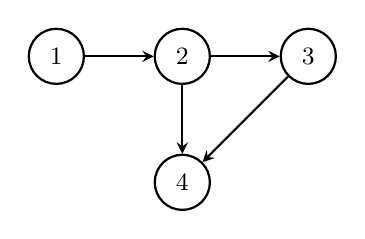
\begin{tikzpicture}[
        node distance=1.6cm, >=stealth, thick,
        every node/.style={circle, draw, minimum size=7mm, font=\small}
      ]
        \node (1) {1};
        \node (2) [right of=1] {2};
        \node (3) [right of=2] {3};
        \node (4) [below of=2] {4};
        \draw[->] (1) -- (2);
        \draw[->] (2) -- (3);
        \draw[->] (2) -- (4);
        \draw[->] (3) -- (4);
      \end{tikzpicture}

      \bigskip
      \small
      $P = \begin{pmatrix}
        0 & 1 & 0 & 0\\
        0 & 0 & \frac{1}{2} & \frac{1}{2}\\
        0 & 0 & 0 & 1\\
        0 & 0 & 0 & 0
      \end{pmatrix}$
    \end{column}
  \end{columns}
\end{frame}

%─────────────────────────────────────────
\begin{frame}{Step 2: Travel-Time Self-Loops}
  \begin{columns}[T]
    \begin{column}{0.52\textwidth}
      \textbf{Problem:} Standard PageRank treats every
      road transition as instantaneous.

      \medskip
      \textbf{Fix:} Add a \highlight{self-loop} proportional to
      traversal time:
      \[
        \boxed{w_i = \mu \cdot \frac{\ell_i}{s_i}}
      \]
      \vspace{-6pt}
      \begin{itemize}\itemsep2pt
        \item $\ell_i$ = road length, $s_i$ = speed limit
        \item $\mu = 20$ = dwell-time scale
      \end{itemize}
      \good{Longer roads trap more mass}
    \end{column}
    \begin{column}{0.45\textwidth}
      
\includegraphics[width=\textwidth]{fig1_selfloop_prob.png}
    \end{column}
  \end{columns}
\end{frame}

%─────────────────────────────────────────
\begin{frame}{Self-Loop: Before \& After}
  \centering
  
\includegraphics[width=0.78\textwidth]{fig9_before_after.png}

  \medskip
  \small Without self-loops: uniform diffusion.\quad
  With self-loops: \good{concentrates on arterials}.
\end{frame}

%─────────────────────────────────────────
\begin{frame}{Step 3: Two-Phase Block Matrix}
  \begin{columns}[T]
    \begin{column}{0.50\textwidth}
      Split each link into two states:
      \begin{itemize}
        \item \highlight{Up} = actively driving through
        \item \highlight{Down} = locally dispersing
      \end{itemize}

      \bigskip
      Block structure ($2N \times 2N$):
      \[
        M_{2N} = \begin{pmatrix}
          (1-\beta)\,P_{\text{self}} & \beta\,I\\
          0 & P_{\text{adj}}
        \end{pmatrix}
      \]

      \begin{itemize}
        \item $\beta = 0.90$: drop-rate to Down phase
        \item $P_{\text{self}}$: includes self-loops
        \item $P_{\text{adj}}$: local adjacency
      \end{itemize}
    \end{column}
    \begin{column}{0.47\textwidth}
      
\includegraphics[width=\textwidth]{fig5_block_matrix.png}
    \end{column}
  \end{columns}
\end{frame}

%─────────────────────────────────────────
\begin{frame}{Key Point: Transition Matrix Uses \underline{No} Ground Truth}
  \centering
  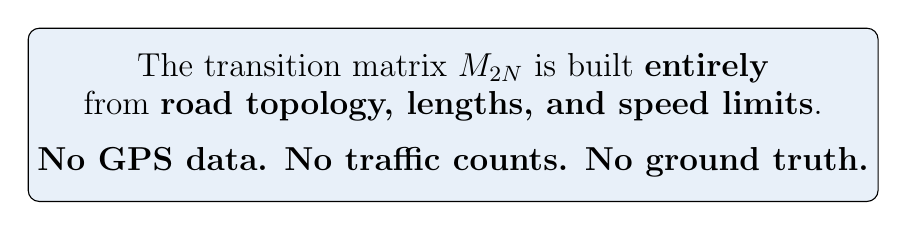
\begin{tikzpicture}
    \node[draw, rounded corners, fill=accent!10, minimum width=10cm,
          minimum height=2.2cm, align=center, font=\large] {
      The transition matrix $M_{2N}$ is built \textbf{entirely}\\
      from \textbf{road topology, lengths, and speed limits}.\\[6pt]
      \textbf{No GPS data.  No traffic counts.  No ground truth.}
    };
  \end{tikzpicture}

  \bigskip
  \begin{tabular}{lll}
    \toprule
    \textbf{Component} & \textbf{Data source} & \textbf{Role}\\
    \midrule
    Transition $M_{2N}$ & Road network (static) & Where vehicles \textbf{move}\\
    Teleportation $E_{2N}$ & GPS data (dynamic) & Where vehicles are \textbf{born}\\
    \bottomrule
  \end{tabular}
\end{frame}

%=================================================================
\section{Building the Teleportation Vector $E_N$}
%=================================================================

%─────────────────────────────────────────
\begin{frame}{Four-Step Construction of $E_N$}
  \begin{enumerate}
    \item \textbf{Extract raw GPS counts} $\mathbf{c} \in \mathbb{Z}_{\geq 0}^N$
          \hfill {\small (most $c_i = 0$)}
    \item \textbf{Laplace pseudo-count:}
          $\tilde{c}_i = c_i + 0.1$
          \hfill {\small (eliminate zeros)}
    \item \textbf{Graph-diffusion smoothing ($\gamma = 0.26$):}
      \[
        c_{\text{smooth}} = 0.74\,\tilde{\mathbf{c}}
        + 0.26\,P_{\text{adj}}\,\tilde{\mathbf{c}}
      \]
    \item \textbf{$L^1$-normalise:}
      \[
        E_N[i] = \frac{c_{\text{smooth},i}}{\sum_j c_{\text{smooth},j}},
        \qquad \sum_i E_N[i] = 1
      \]
  \end{enumerate}

  \bigskip
  \begin{block}{Result}
    $E_N[i]$ = probability that a new vehicle appears on link $i$
  \end{block}
\end{frame}

%─────────────────────────────────────────
\begin{frame}{Worked Example: 5-Link Network}
  \centering
  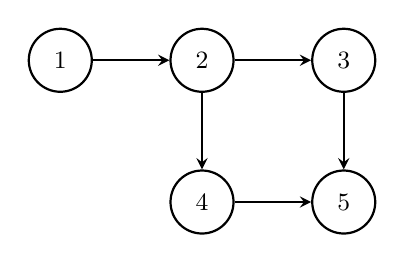
\begin{tikzpicture}[
    node distance=1.8cm, >=stealth, thick,
    every node/.style={circle, draw, minimum size=8mm, font=\small}
  ]
    \node (1) {1};
    \node (2) [right of=1] {2};
    \node (3) [right of=2] {3};
    \node (4) [below of=2] {4};
    \node (5) [right of=4] {5};
    \draw[->] (1) -- (2);
    \draw[->] (2) -- (3);
    \draw[->] (2) -- (4);
    \draw[->] (3) -- (5);
    \draw[->] (4) -- (5);
  \end{tikzpicture}

  \bigskip
  \small
  \begin{tabular}{lccccc}
    \toprule
    & Link 1 & Link 2 & Link 3 & Link 4 & Link 5\\
    \midrule
    Raw count $c_i$ & 0 & 5 & 0 & 3 & 0\\
    + Laplace $\tilde{c}_i$ & 0.10 & 5.10 & 0.10 & 3.10 & 0.10\\
    Neighbour avg & 5.10 & 1.60 & 0.10 & 0.10 & ---\\
    Smoothed & 1.40 & 4.19 & 0.10 & 2.32 & 0.10\\
    \highlight{$E_N[i]$} & \highlight{0.172} & \highlight{0.516}
      & \highlight{0.012} & \highlight{0.286} & \highlight{0.012}\\
    \bottomrule
  \end{tabular}

  \medskip
  Link~1 gets \good{17.2\%} despite zero observations
  $\Rightarrow$ topology propagates evidence from its busy neighbour
\end{frame}

%─────────────────────────────────────────
\begin{frame}{Extending to $2N$: The $E_{2N}$ Vector}
  Teleportation injects vehicles only into the \highlight{Up (active)} phase:
  \[
    \boxed{E_{2N} = \begin{pmatrix} E_N \\ \mathbf{0}_N \end{pmatrix}}
    \in \mathbb{R}^{2N}, \qquad \|E_{2N}\|_1 = 1
  \]

  \bigskip
  \textbf{Physical meaning:}
  \begin{itemize}
    \item New vehicles ``start'' actively driving on a road
    \item They naturally transition to the Down phase over time
    \item No vehicles are born directly into local dispersal mode
  \end{itemize}
\end{frame}

%=================================================================
\section{The PageRank Power Iteration}
%=================================================================

%─────────────────────────────────────────
\begin{frame}{Combining Topology + Ground Truth}
  \begin{block}{\large The Power Iteration}
    \[
      \boxed{\mathbf{v}^{(k+1)}
      = \underbrace{d \cdot M_{2N}^\top \cdot \mathbf{v}^{(k)}}_{\text{topology (80\%)}}
      + \underbrace{(1-d) \cdot E_{2N}}_{\text{ground truth (20\%)}}}
    \]
  \end{block}

  \bigskip
  \begin{columns}[T]
    \begin{column}{0.48\textwidth}
      \centering\highlight{$d = 0.80$}\\[4pt]
      80\% of mass follows the\\
      \textbf{transition matrix}\\
      (roads, speeds, physics)
    \end{column}
    \begin{column}{0.48\textwidth}
      \centering\highlight{$1 - d = 0.20$}\\[4pt]
      20\% of mass is re-injected\\
      from \textbf{ground truth GPS}\\
      (observed traffic pattern)
    \end{column}
  \end{columns}

  \bigskip
  \centering
  Iterate until $\|\mathbf{v}^{(k+1)} - \mathbf{v}^{(k)}\|_1 < 10^{-6}$
\end{frame}

%─────────────────────────────────────────
\begin{frame}{Convergence}
  \centering
  
\includegraphics[width=0.68\textwidth]{fig10_convergence.png}

  \small Typically converges in $\sim$40--60 iterations.
\end{frame}

%=================================================================
\section{Smoothing Justification}
%=================================================================

%─────────────────────────────────────────
\begin{frame}{Why Smooth? --- The Sparsity Problem}
  \begin{columns}[T]
    \begin{column}{0.45\textwidth}
      \begin{itemize}
        \item Most links have $c_i = 0$
        \item Creates:
          \begin{itemize}
            \item MRE singularities
            \item Markov chain dead zones
            \item Biased teleportation
          \end{itemize}
        \item Without smoothing:\\
          \bad{MRE = 7{,}275}
        \item With smoothing:\\
          \good{MRE = 0.19}
      \end{itemize}
    \end{column}
    \begin{column}{0.52\textwidth}
      
\includegraphics[width=\textwidth]{fig11_sparsity_histogram.png}
    \end{column}
  \end{columns}
\end{frame}

%─────────────────────────────────────────
\begin{frame}{Graph-Diffusion as a Low-Pass Filter}
  \[
    \mathbf{c}_{\text{smooth}}
    = \underbrace{(1-\gamma)}_{\text{keep own}}
      \cdot \tilde{\mathbf{c}}
    + \underbrace{\gamma}_{\text{borrow from neighbours}}
      \cdot P_{\text{adj}}\,\tilde{\mathbf{c}}
  \]

  \bigskip
  \begin{columns}[T]
    \begin{column}{0.48\textwidth}
      \centering
      \textbf{Spectral view:}\\[6pt]
      Eigenvalue of the filter:
      \[
        h(\lambda) = (1-\gamma) + \gamma\lambda
      \]
      $h(1) = 1$ \good{(preserves mean)}\\
      $h(-1) = 1-2\gamma$ \good{(attenuates noise)}
    \end{column}
    \begin{column}{0.48\textwidth}
      \centering
      \textbf{Mass conservation:}\\[6pt]
      \[
        \sum_i c_{\text{smooth},i} = \sum_i \tilde{c}_i
      \]
      Smoothing \textbf{redistributes}\\
      mass but never creates\\
      or destroys it
    \end{column}
  \end{columns}
\end{frame}

%─────────────────────────────────────────
\begin{frame}{The Bias-Variance Tradeoff}
  \begin{columns}[T]
    \begin{column}{0.42\textwidth}
      \[
        \text{MSE} = \underbrace{\text{Bias}^2}_{\uparrow\;\text{with}\;\gamma}
        + \underbrace{\text{Variance}}_{\downarrow\;\text{with}\;\gamma}
      \]
      \begin{itemize}
        \item Too little smoothing $\to$ \bad{noisy}
        \item Too much smoothing $\to$ \bad{blurred}
        \item U-shaped MSE curve
        \item Minimum \textbf{inside} the range
      \end{itemize}
    \end{column}
    \begin{column}{0.55\textwidth}
      
\includegraphics[width=\textwidth]{fig14_bias_variance_decomp.png}
    \end{column}
  \end{columns}
\end{frame}

%─────────────────────────────────────────
\begin{frame}{Cross-Validation Protocol (49 Trials)}
  \begin{enumerate}
    \item Select 49 timeframe slots (fixed seed = 42)
    \item \textbf{Split} GPS data: Set~A (train) / Set~B (test)
    \item Smooth Set~A with candidate $\gamma$
    \item \textbf{Never} smooth Set~B (oracle ground truth)
    \item Measure:
      \begin{itemize}
        \item \highlight{Predictive MSE}: smoothed A vs.\ raw B
        \item \highlight{PageRank MSE}: PageRank(A) vs.\ PageRank(B)
        \item \highlight{Pearson $r$}: correlation A vs.\ B
      \end{itemize}
    \item Average over all 49 trials
  \end{enumerate}
\end{frame}

%─────────────────────────────────────────
\begin{frame}{CV Results: MSE \& Correlation}
  \centering
  
\includegraphics[width=0.75\textwidth]{fig12_cv_mse_correlation.png}

  \medskip
  Both metrics optimised at \highlight{$\gamma^* = 0.26$}
\end{frame}

%─────────────────────────────────────────
\begin{frame}{CV Results: Downstream PageRank}
  \centering
  
\includegraphics[width=0.75\textwidth]{fig13_cv_downstream_variance.png}

  \medskip
  PageRank MSE minimum \textbf{also} at $\gamma \approx 0.26$
  $\Rightarrow$ input-optimal = output-optimal
\end{frame}

%─────────────────────────────────────────
\begin{frame}{Direct vs.\ Downstream MSE}
  \centering
  
\includegraphics[width=0.82\textwidth]{fig6_smoothing_tradeoff.png}
\end{frame}

%─────────────────────────────────────────
\begin{frame}{Independent Verification (Seed = 123, 80 Splits)}
  \centering
  
\includegraphics[width=0.82\textwidth]{fig16_verification.png}

  \bigskip
  \small Broad plateau at $\gamma \in [0.22, 0.30]$;
  $\gamma = 0.26$ is the \good{centre of the plateau}.\\
  MSE varies $<0.04\%$ within this band.
\end{frame}

%=================================================================
\section{Results}
%=================================================================

%─────────────────────────────────────────
\begin{frame}{Impact of Smoothing: 490-Timeframe Comparison}
  \centering
  
\includegraphics[width=0.80\textwidth]{fig15_raw_vs_smoothed_mre.png}

  \medskip
  \small
  \begin{tabular}{lcc}
    \toprule
    Pipeline & Avg MRE & Improvement\\
    \midrule
    Raw ($\gamma = 0$) & \bad{7,275} & ---\\
    Smoothed ($\gamma = 0.26$) & \good{0.19} & $\times$37,800\\
    \bottomrule
  \end{tabular}
\end{frame}

%─────────────────────────────────────────
\begin{frame}{Effect of $\mu$ (Dwell-Time Scale)}
  \centering
  
\includegraphics[width=0.68\textwidth]{fig4_mre_vs_mu.png}

  \medskip
  MRE drops monotonically as $\mu$ increases.
  Optimal: \highlight{$\mu = 20$}
\end{frame}

%─────────────────────────────────────────
\begin{frame}{MRE Heatmap: $\mu$ vs $\beta$}
  \centering
  
\includegraphics[width=0.62\textwidth]{fig3_mre_heatmap.png}

  \medskip
  Best: $\mu = 20$, $\beta = 0.90$, $d = 0.80$
\end{frame}

%─────────────────────────────────────────
\begin{frame}{Damping Sensitivity}
  \centering
  
\includegraphics[width=0.68\textwidth]{fig8_damping_sensitivity.png}

  \medskip
  $d = 0.80$ balances topology-driven flow
  with ground-truth injection
\end{frame}

%=================================================================
\section{Summary}
%=================================================================

%─────────────────────────────────────────
\begin{frame}{The Four Tuneable Parameters}
  \centering
  \begin{tabular}{clcl}
    \toprule
    Symbol & Name & Value & Controls\\
    \midrule
    $\gamma$ & Smoothing & 0.26 & Evidence propagation strength\\
    $\mu$ & Dwell-time & 20 & Self-loop weight (road physics)\\
    $\beta$ & Phase-drop & 0.90 & Active $\to$ dispersal rate\\
    $d$ & Damping & 0.80 & Topology vs.\ ground truth\\
    \bottomrule
  \end{tabular}

  \bigskip
  \begin{block}{Transferability}
    For a new city: get road network $+$ some GPS data $\to$
    grid-search over $(\gamma, \mu, \beta, d)$
  \end{block}
\end{frame}

%─────────────────────────────────────────
\begin{frame}{Key Takeaways}
  \begin{enumerate}
    \item \highlight{Transition matrix} $M_{2N}$ uses \textbf{only topology}\\
          (road graph $+$ lengths $+$ speeds)
    \bigskip
    \item \highlight{Teleportation vector} $E_{2N}$ uses \textbf{only ground truth}\\
          (GPS counts $\to$ Laplace $\to$ smoothing $\to$ normalise)
    \bigskip
    \item \highlight{Smoothing is justified} by cross-validation:\\
          $\gamma^* = 0.26$ minimises MSE (interior minimum, not boundary)
    \bigskip
    \item \highlight{Result}: MRE improves from 7,275 $\to$ 0.19\\
          ($37{,}800\times$ improvement with smoothing alone)
  \end{enumerate}
\end{frame}

%─────────────────────────────────────────
\begin{frame}{}
  \centering
  \vfill
  {\Huge\highlight{Thank You}}

  \vfill
  {\large Questions?}
  \vfill
\end{frame}

\end{document}
